\documentclass{article}
\usepackage[utf8]{inputenc}
\usepackage[T1]{fontenc}
\usepackage[english]{babel}
\setlength{\parindent}{0pt}
\usepackage{hyperref}
\hypersetup{
    colorlinks=true,
    linkcolor=blue,
    filecolor=magenta,      
    urlcolor=cyan,
    pdftitle={Sharelatex Example},
    pdfpagemode=FullScreen}
\usepackage{graphicx}
\graphicspath{ {./pic/} }

\usepackage{fourier,amssymb,microtype,amsmath,gensymb}
\newcommand{\R}{\mathbb{R}}
\usepackage{mdframed,caption,xcolor}
\usepackage{tikz,tkz-euclide}

\title{Questions and Answers}
\author{Xiaoguang Ling \\  \href{xiaoguang.ling@econ.uio.no}{xiaoguang.ling@econ.uio.no}}
\date{\today}

\begin{document}

\maketitle

\tableofcontents

\newpage
%%%%%%%%%%%%%%%%%%%%%%%%%%%%%%%%%%%%%%%%%%%%%%%%%%%%%%%%%%%%%%%%%%%%%%%%%%%%%%%%%%%%%%%%%%%%%%
\section{Seminar 1}

%***************************************************
\subsection{question 1.26}

Q: Should it be "equality" in Kuhn-Tucker condition equation (6): $p_1x_1 + p_2x_2 \le y$ (slides pp.16)?

\vspace{2mm}

A: You can argue it is "equality" for a well defined
classical utility function, since the solution is always
on the boundary(you can always spend the rest part of your
budget to imporve your utility).

But note that Kuhn-Tucker condition describes the most
general case for a value maximization problem. If the 
utility function is weired, for example, in Figure \ref{fig:ktc},
the utility function ($u(x_1,x_2) =3-\left(x_1-2\right)^2-\left(x_2-2\right)^2$) looks like a cone, the "peak" of the cone
is within the "budget plane($x+y=6$)". Your utility can therefore be maximized within your budget. "$\le$" allows this case.

\vspace{2mm}

{\centering
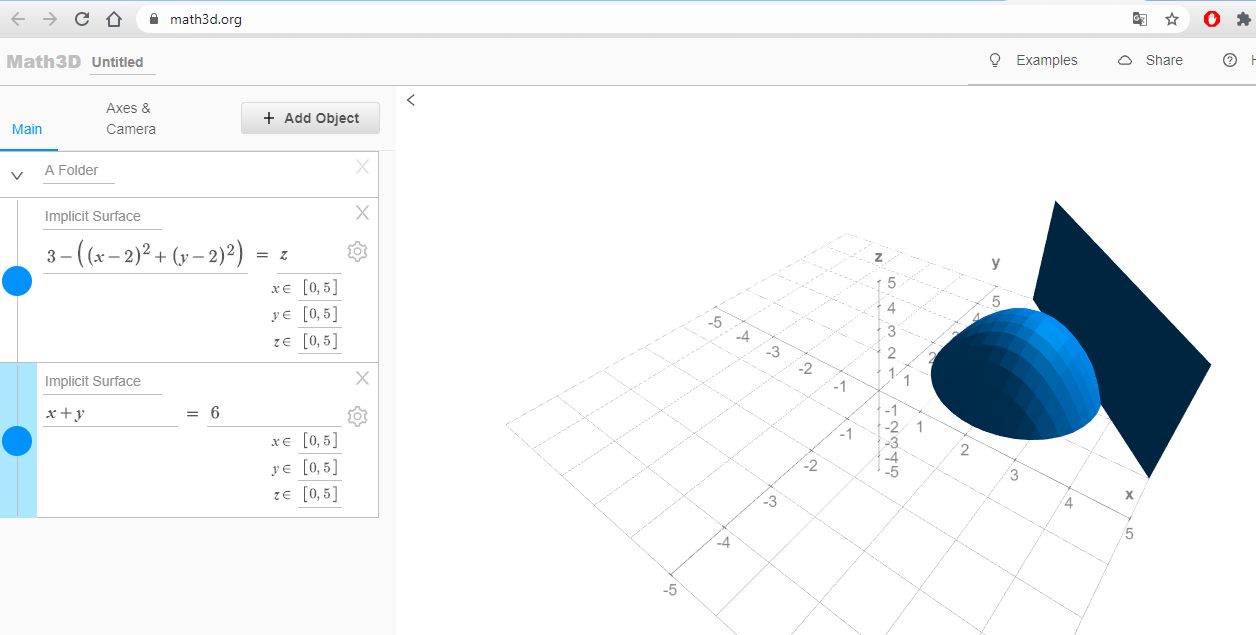
\includegraphics[width=1\textwidth]{1.q_ktc}
\captionof{figure}{A cone-like utility function and a loose budget}
\label{fig:ktc}}

\vspace{2mm}

Try to make some graphs yourself on \href{https://www.math3d.org/}{https://www.math3d.org/}. Always remember your utility is the 
extra dimension (z-axis in Figure \ref{fig:ktc}).


%%%%%%%%%%%%%%%%%%%%%%%%%%%%%%%%%%%%%%%%%%%%%%%%%%%%%%%%%%%%%%%%%%%%%%%%%%%%%%%%%%%%%%%%%%%%%%
\section{Seminar 2}


%%%%%%%%%%%%%%%%%%%%%%%%%%%%%%%%%%%%%%%%%%%%%%%%%%%%%%%%%%%%%%%%%%%%%%%%%%%%%%%%%%%%%%%%%%%%%%
\section{Previous exams}

\subsection{Cost minimization}

Q: The competitive firm FF has a production function of the form:
$F = 2L + 5K$, where $L$ denotes labor and $K$ capital. Assume salary $w=2$ and capital cost is $r=4$. What is the minimal cost of producing 10 units of output?

(It's from \href{https://www.uio.no/studier/emner/sv/oekonomi/ECON3200/previous-exams/econ32_4200-2019v-sensorveiledning.pdf}{Spring 2019 Exam})

\bigskip
A: You can solve it in the following 3 ways:

\medskip

\textbf{1. Kuhn Tucker condition (not recommended)}

In this question, you're going to solve the cost minimization problem: $\min 2L + 4K , s.t. \  f(x) > = 10, L\ge0, K\ge0$. \\
You can definitely use Kuhn Tucker condition to solve it, similar to the question in our seminar 1, since the object function is also linear. 

\bigskip

\textbf{2. Substitute the constraint into the object function (be careful with the domain)}

Since you're going to minimize the cost, it's not reasonable to produce more than required (i.e. $10$, because cost function is increasing in output y), you will let $f(x)=10$, i.e. $F= 2L+5K=10$, or $2L=10-5K$.​ This relation holds as long as you want to minimize the cost. 
\medskip

Also, don't forget you have  $L\ge0$ and $K\ge0$.  Thus $2L=10-5K$ must also be non-negative, we have $10-5K \ge0, K\le2$. The domain of $K$ is $[0,2]$ \\
You can now substitute $2L=10-5K$ into your object function, $2L+4K$, and your minimization problem​ becomes $\min 10-5K +4K$ , or $\min 10 - K$. The object function is decreasing in K,  you want K to be as great as possible in its domain $[0,2]$, to minimize the cost. \\
So you choose $K=2, L=0$, minimized cost is $8$.
\medskip

In exam, you can write it concisely:
\medskip

 $\min 2L + 4K \  s.t. \  f(x) > = 10, L\ge0, K\ge0$ \\
Since cost function is increasing in output, $f(x)=10, i.e. \  F= 2L+5K=10$. Therefore: $2L=10-5K$.  Objection function becomes: 10-5K+4K=10-K, decreasing in K. \\
Besides, $K\ge0,  L\ge0$ and $2L=10-5K$  lead to $K \in [0,2]$. \\
Therefore $K^*=2, L^*=0$, 

\bigskip

\textbf{3. Cheapest per unit of product (recommended)}

Since the production function shows perfect substitution between $L$ and $K$, the firm chooses only the cheapest per unit of product input. Recall that perfect substitution means $K$ and $L$ are the same thing, just with different package, in the view of the firm.

\medskip
To produce $1$ unit output, according to $F = 2L+5K$, you need either $0.5$ unit $L$ or $0.2$ unit $K$. The price for $0.5$ unit $L$ is $0.5 \times 2 =1$; the price for $0.2$ unit $K​$ is $0.2 \times 4 =0.8$.
For $1$ unit output, $K$ is the cheapest input. Therefore the firm chooses $L=0, F=5K$. When $F=10$, $K=2$, the cost is $2 \times 4 =8$.







\end{document}
